\documentclass[a4paper,11pt]{article}
\usepackage[T1]{fontenc}
\usepackage[utf8]{inputenc}
\usepackage{lmodern}
\usepackage{hyperref}
\usepackage{graphicx}
\usepackage[english]{babel}
\newenvironment{dedication}
{
   \cleardoublepage
   \thispagestyle{empty}
   \vspace*{\stretch{1}}
   \hfill\begin{minipage}[t]{0.66\textwidth}
   \raggedright
}
{
   \end{minipage}
   \vspace*{\stretch{3}}
   \clearpage
}

\makeatletter
%\renewcommand{\@chapapp}{}% Not necessary...
\newenvironment{chapquote}[2][2em]
  {\setlength{\@tempdima}{#1}%
   \def\chapquote@author{#2}%
   \parshape 1 \@tempdima \dimexpr\textwidth-2\@tempdima\relax%
   \itshape}
  {\par\normalfont\hfill--\ \chapquote@author\hspace*{\@tempdima}\par\bigskip}
\makeatother
\title{\Huge \textbf{\v{S}ifrovanje elektronske po\v{s}te za MacOSX}}

\author{\textsc{Cryptoparty Serbia}}
\begin{document}


%\frontmatter
\maketitle
\tableofcontents

%\mainmatter
\newpage

\section{Kratak uvod}
Ovo uputstvo \'{c}e vam pokazati kako da \v{s}ifrujete elektronsku po\v{s}tu na operativnom sistemu Mekinto\v{s} koriste\'{c}i podrazumevanog klijenta elektronske po\v{s}te tj. imejl klijenta na Mekinto\v{s}u.\newline
Mekino\v{s} operatini sistem nije u potpunosti otvorenog koda, kao ni softver koji dolazi uz operativni sistem, pa ne treba imati previ\v{s}e poverenja u privatnost li\v{c}nih podataka na ovom operativnom sistemu.
Kada je to re\v{c}eno pre\dj{}imo na uputstvo za konfigurisanje \textbf{GPG} programa za Mac.
\newpage
\section{Instlacija GpgTools programa}
Najpre je potrebno da preuzmete prgram \textbf{GpgTools} sa \href{https://gpgtools.org}{gpgtools.org}. \newline
To je program zadu\v{z}en za kreiranje \textbf{GPG} klju\v{c}eva potrebnih za \textsf{\v{s}ifrovanje} \textsf{de\v{s}ifrovanje} poruka, \textsf{digitalno potpisivanje} i \textsf{provere digitalnih potpisa} poruka.

\begin{figure}[!h]
	\begin{center}
		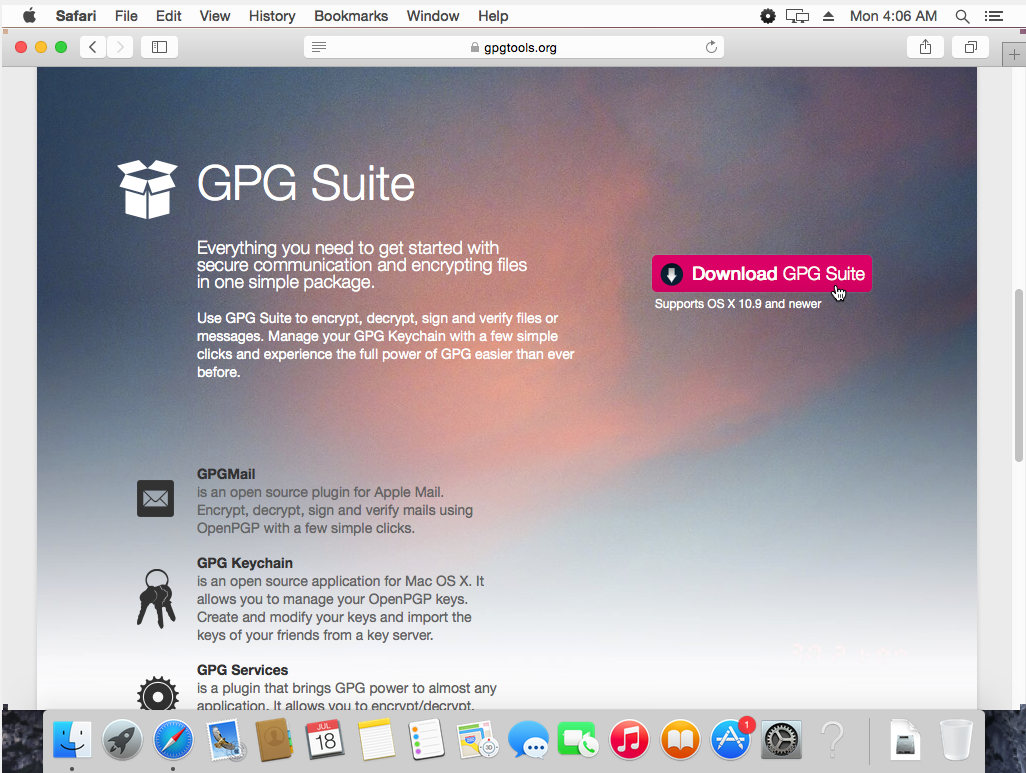
\includegraphics[width=8cm]{01_Oracle_VM_VirtualBox.png}
		\caption{Preuzmite GpgTools sa interneta}
		\label{gpgtools_download1}
	\end{center}
\end{figure}

\begin{figure}[!h]
	\begin{center}
		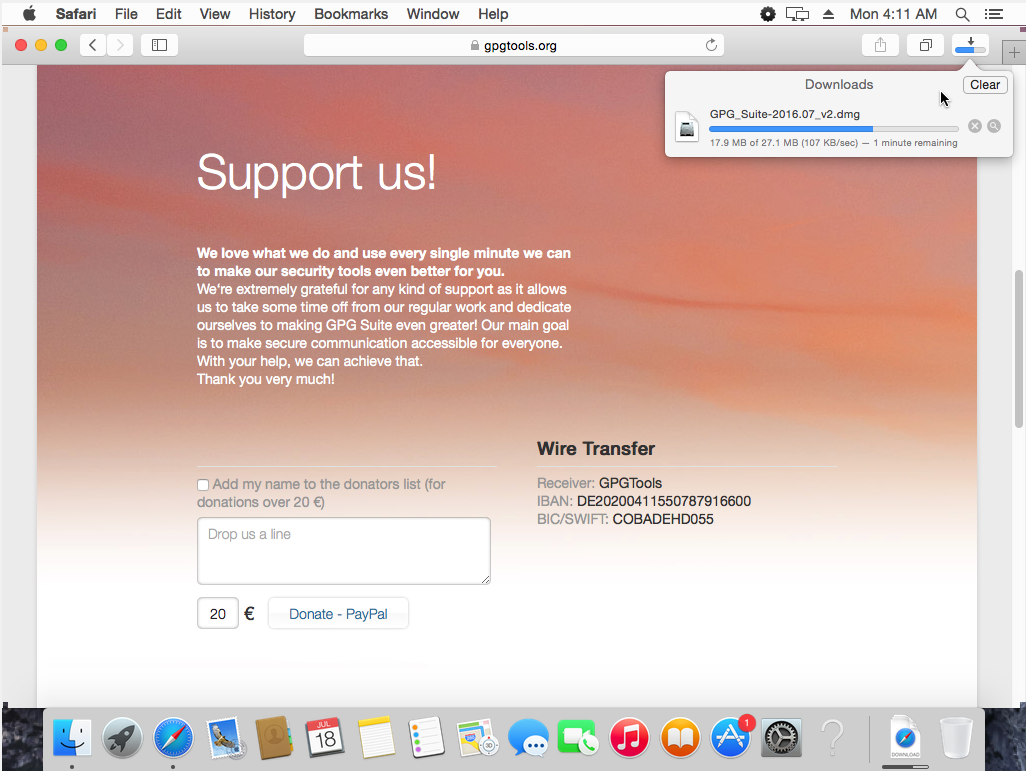
\includegraphics[width=8cm]{02_Oracle_VM_VirtualBox.png}
		\caption{Kada se zavr\v{s}i preuzimanje \textbf{Gpgtools} programa, pokrenite ga.}
		\label{gpgtools_download2}
	\end{center}
\end{figure}
\newpage

\begin{figure}[!h]
	\begin{center}
		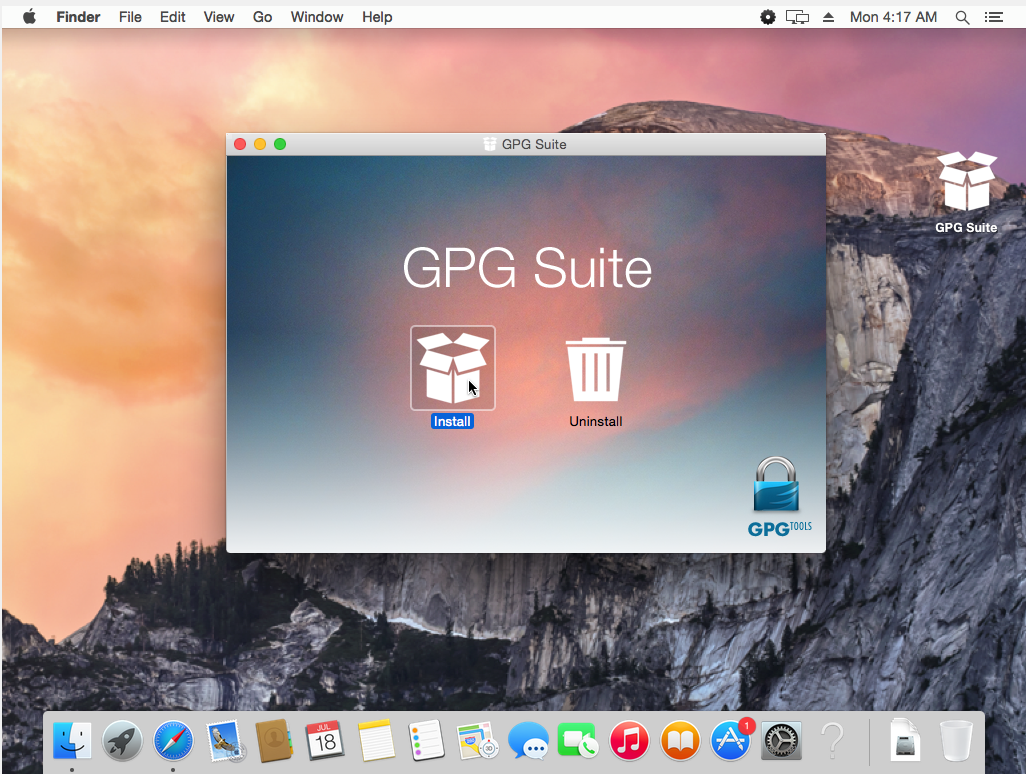
\includegraphics[width=8cm]{03_Oracle_VM_VirtualBox.png}
		\caption{Po pokretanju \textbf{Gpgtools} programa idaberite \textbf{Install} opciju da bi ste intsalirali program}
		\label{gpgtools_install1}
	\end{center}
\end{figure}

\begin{figure}[!h]
	\begin{center}
		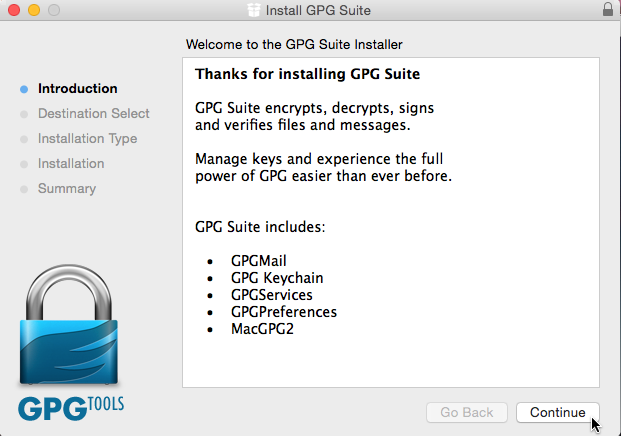
\includegraphics[width=8cm]{04_Oracle_VM_VirtualBox.png}
		\caption{Pro\dj{}ite kroz jednostavan proces instalacije..}
		\label{gpgtools_install2}
	\end{center}
\end{figure}
\newpage
\begin{figure}[!h]
	\begin{center}
		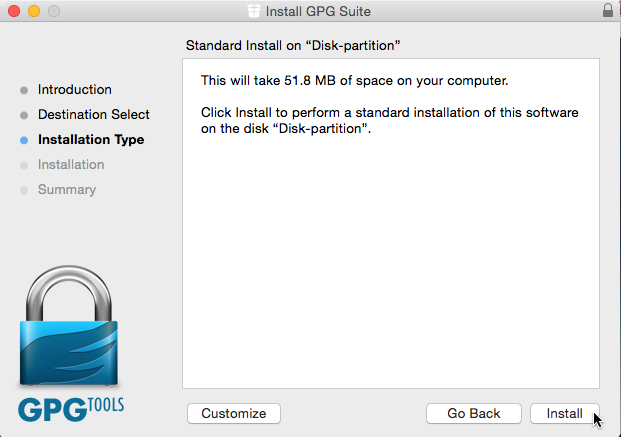
\includegraphics[width=8cm]{05_Oracle_VM_VirtualBox.png}
		\caption{standardna instalacija \'{c}e uraditi sve potrebno za vas automatski.}
		\label{gpgtools_install3}
	\end{center}
\end{figure}

\begin{figure}[!h]
	\begin{center}
		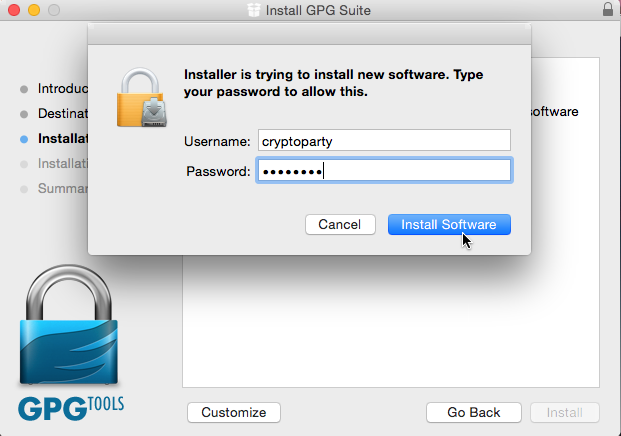
\includegraphics[width=8cm]{06_Oracle_VM_VirtualBox.png}
		\caption{Naravno, tra\v{z}i\'{c}e vam \v{s}ifru korisnika sistema kako bi se program instalirao.}
		\label{gpgtools_install4}
	\end{center}
\end{figure}
\newpage
\begin{figure}[!h]
	\begin{center}
		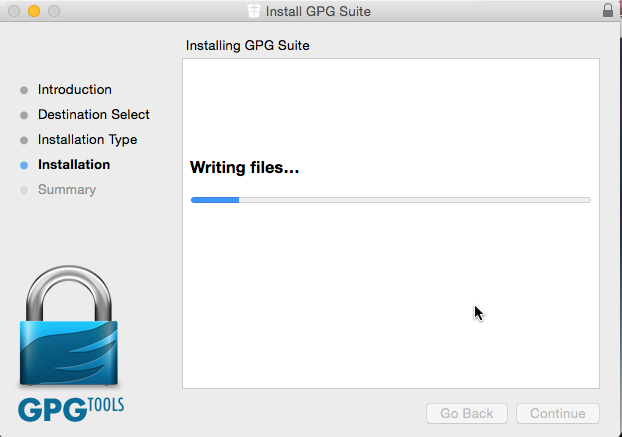
\includegraphics[width=8cm]{07_Oracle_VM_VirtualBox.png}
		\caption{I kada zavr\v{s}i sa upisom podataka proces instalacije je gotov.}
		\label{gpgtools_install5}
	\end{center}
\end{figure}
\newpage
\subsection{Generisanje GPG klju\v{c}eva}
\begin{figure}[!h]
	\begin{center}
		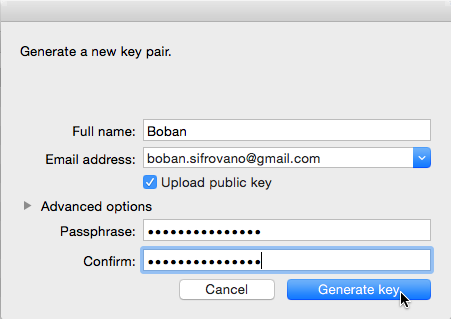
\includegraphics[width=6cm]{08_Oracle_VM_VirtualBox.png}
		\caption{Sada unesite email adresu za koju generi\v{s}ete klju\v{c}eve i podesite \v{s}ifru za te klju\v{c}eve\newline Ovu \v{s}ifru morate zapamtiti ili zapisati negde, jer \'{c}e vam trebati da bi ste de\v{s}ifrovali primljene \v{s}ifrovane poruke.}
		\label{gpgtools_keygen1}
	\end{center}
\end{figure}
\begin{figure}[!h]
	\begin{center}
		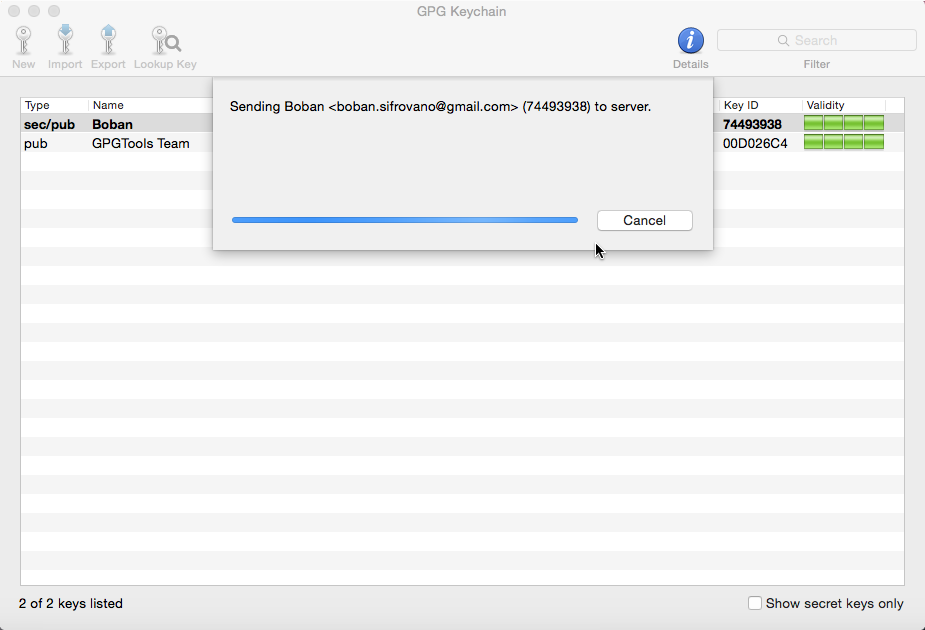
\includegraphics[width=8cm]{09_Oracle_VM_VirtualBox.png}
		\caption{Kada i to zavr\v{s}ite, \textbf{Gpgtools} \'{c}e va\v{s} novi javni klju\v{c} poslati na server javnih klju\v{c}eva kako bi drugi ljudi koristili taj javni klju\v{c} da vam po\v{s}alju \v{s}ifrovane poruke.}
		\label{gpgtools_keygen2}
	\end{center}
\end{figure}
\newpage
\begin{figure}[!h]
	\begin{center}
		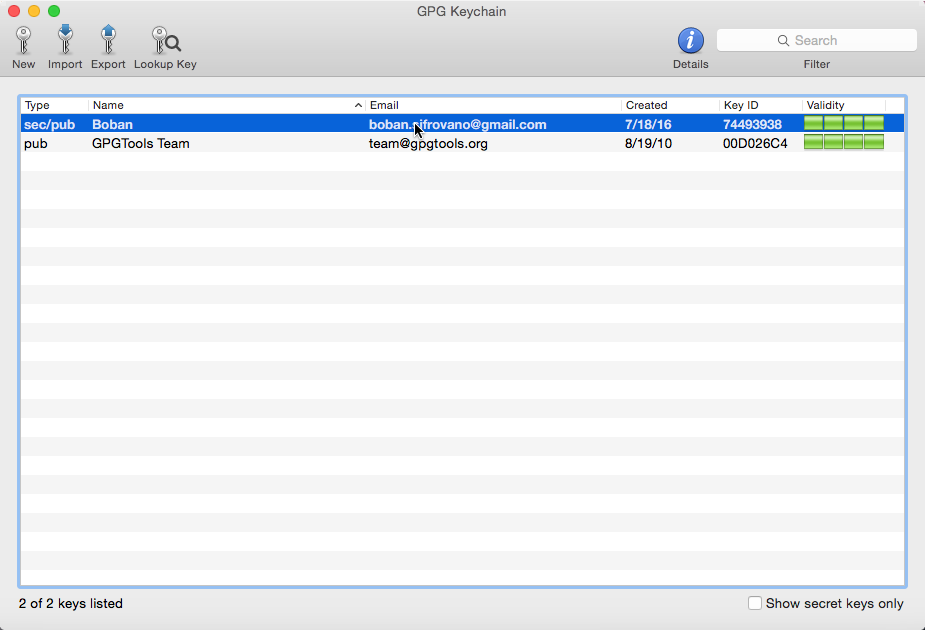
\includegraphics[width=8cm]{10_Oracle_VM_VirtualBox.png}
		\caption{Va\v{s} novi klju\v{c} \'{c}e biti prikazan u \textbf{GpgTools} bazi klju\v{c}eva. }
		\label{gpgtools_keygen3}
	\end{center}
\end{figure}
\begin{figure}[!h]
	\begin{center}
		
\includegraphics[width=8cm]{11_Oracle_VM_VirtualBox.png}
		\caption{Sada je potrebno da podesimo i mejl klijenta za isti mejl nalog za koji smo kreirali klju\v{c}eva, ukoliko to ve\'{c} nismo ranije uradili.}
		\label{gpgtools_email_setup1}
	\end{center}
\end{figure}
\begin{figure}[!h]
	\begin{center}
		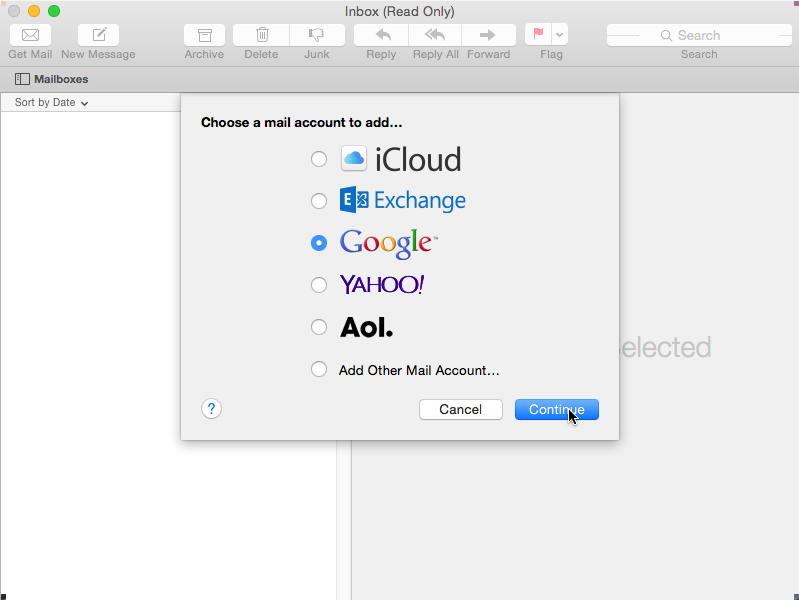
\includegraphics[width=8cm]{12_Oracle_VM_VirtualBox.png}
		\caption{Konkretno mi koristimo Gmail u ovom uputstvu, a vi podesite za va\v{s}eg mejl provajdera. }
		\label{gpgtools_email_setup2}
	\end{center}
\end{figure}
\newpage
\begin{figure}[!h]
	\begin{center}
		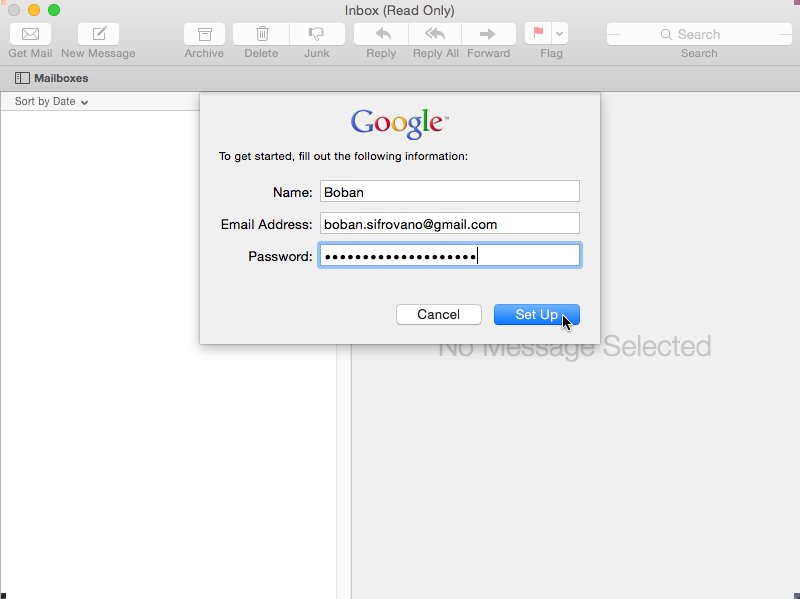
\includegraphics[width=8cm]{13_Oracle_VM_VirtualBox.png}
		\caption{Pdesite istu mejl adresu kao onu za koju ste kreirali klju\v{c}eve.}
		\label{gpgtools_email_setup3}
	\end{center}
\end{figure}
\begin{figure}[!h]
	\begin{center}
		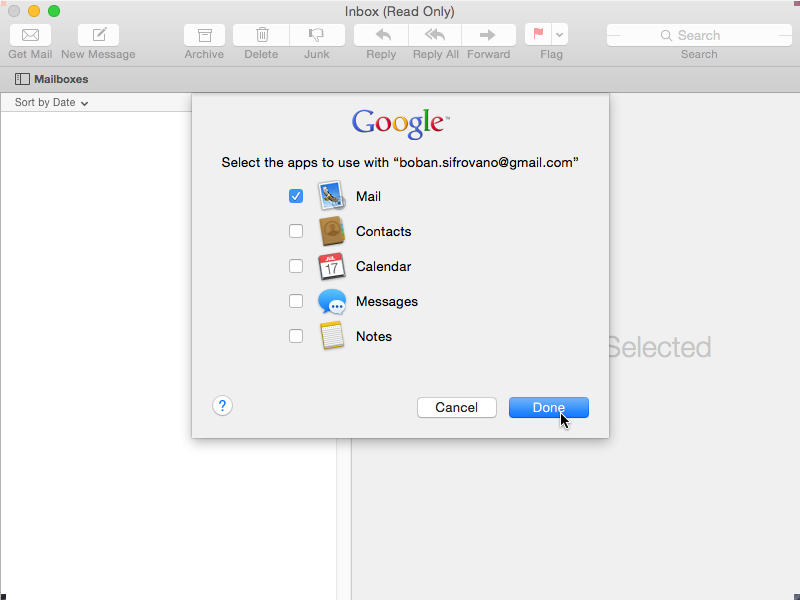
\includegraphics[width=8cm]{14_Oracle_VM_VirtualBox.png}
		\caption{Koristimo mejl naravno.}
		\label{gpgtools_email_setup4}
	\end{center}
\end{figure}
\newpage
\begin{figure}[!h]
	\begin{center}
		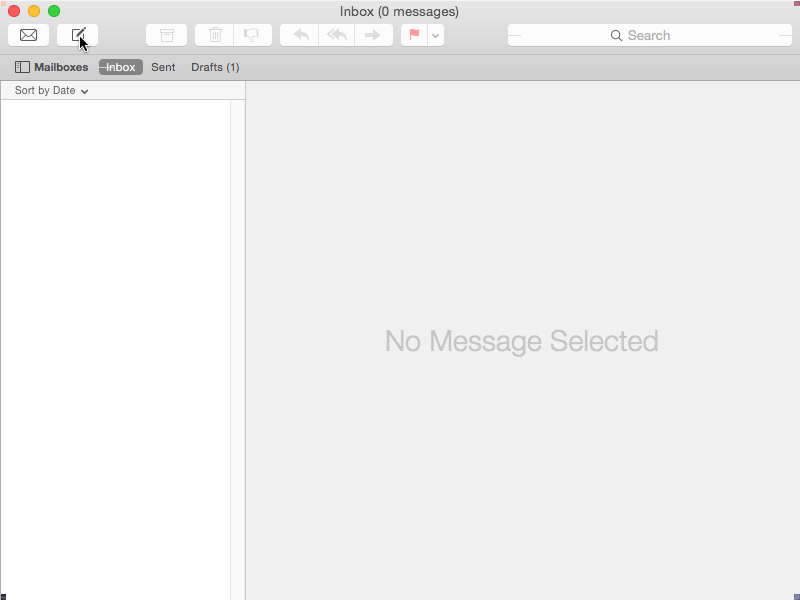
\includegraphics[width=8cm]{15_Oracle_VM_VirtualBox.png}
		\caption{Sada \'{c}e mo poku\v{s}ati da napi\v{s}emo \v{s}ifrovanu poruku.}
		\label{gpgtools_email_setup5}
	\end{center}
\end{figure}
\section{\v{S}ifrovanje poruke primaocu po\v{s}te}
\begin{figure}[!h]
	\begin{center}
		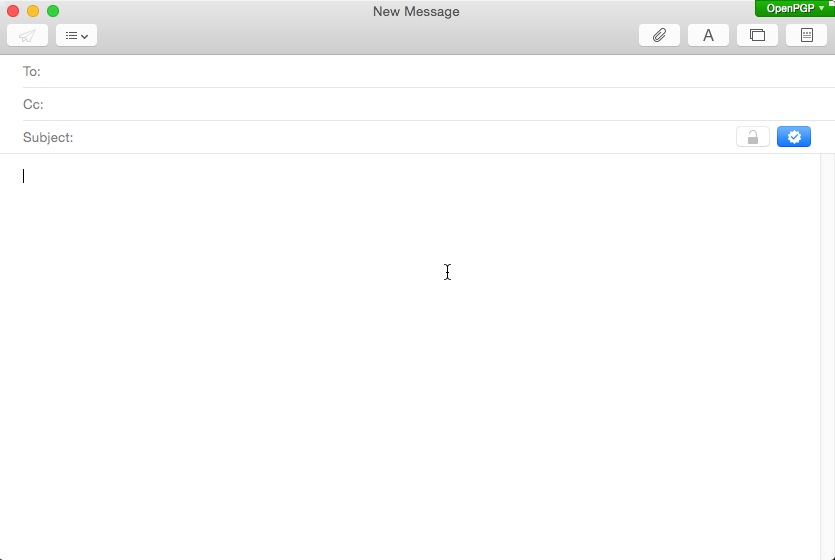
\includegraphics[width=8cm]{16_Oracle_VM_VirtualBox.png}
		\caption{Primetite kako u gornjem desnom uglu prozora za sastavljanje poruke ima zeleni pravouganik sa zankom \textbf{OpenPGP}. To zna\v{c}i da je \textbf{Gpgtools} integrisan u mejl kljijenta. Tako\dj{}e primetite da je sivi katanac otklju\v{c}an. Da bi \v{s}ifrovali poruku za nekog primaoca, prvo moramo imati njegov javni klju\v{c} (ako primaoc koristi GPG tj. ima svoje klju\v{c}eve)}
		\label{gpgtools_email_setup6}
	\end{center}
\end{figure}
\begin{figure}[!h]
	\begin{center}
		
\includegraphics[width=8cm]{17_Oracle_VM_VirtualBox.png}
		\caption{Pa ponovo otvaramo \textbf{Gpgtolls} kako bi smo iz njega tra\v{z}ili javni klju\v{c} osobe kojoj \v{s}ifrujemo mejl.}
		\label{gpgtools_email_setup7}
	\end{center}
\end{figure}
\newpage
\begin{figure}[!h]
	\begin{center}
		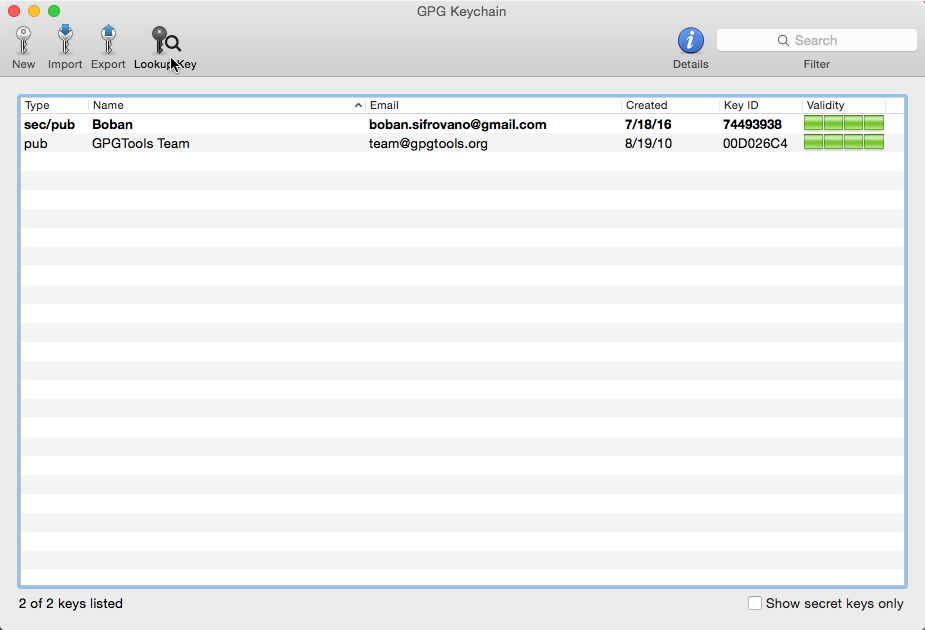
\includegraphics[width=8cm]{18_Oracle_VM_VirtualBox.png}
		\caption{Tra\v{z}imo klju\v{c}eve.}
		\label{gpgtools_email_setup8}
	\end{center}
\end{figure}
\begin{figure}[!h]
	\begin{center}
		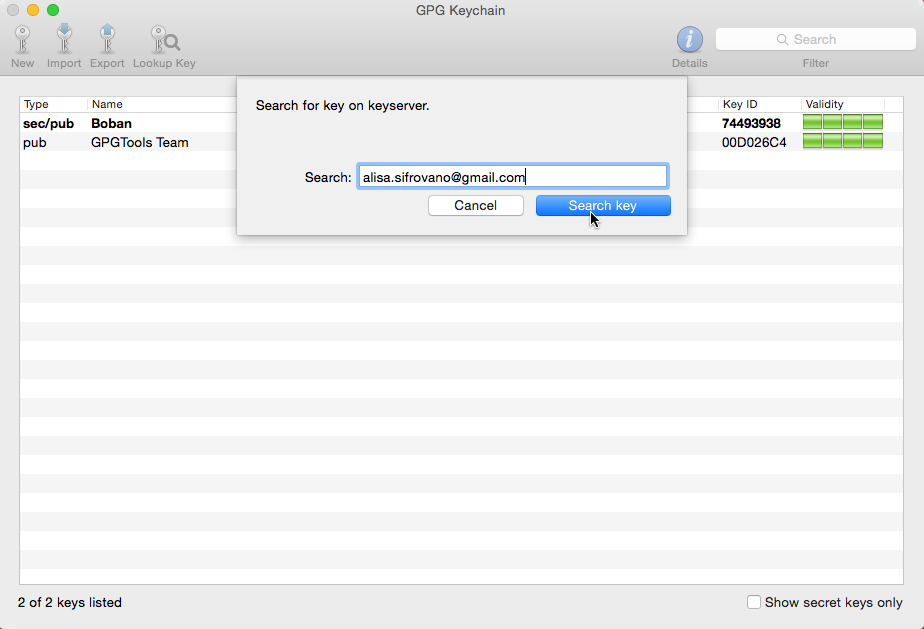
\includegraphics[width=8cm]{19_Oracle_VM_VirtualBox.png}
		\caption{Unosimo mejl adresu ongoa \v{c}iji nam javni klju\v{c} treba, tj onome kome pi\v{s}emo.}
		\label{gpgtools_email_setup9}
	\end{center}
\end{figure}
\newpage
\begin{figure}[!h]
	\begin{center}
		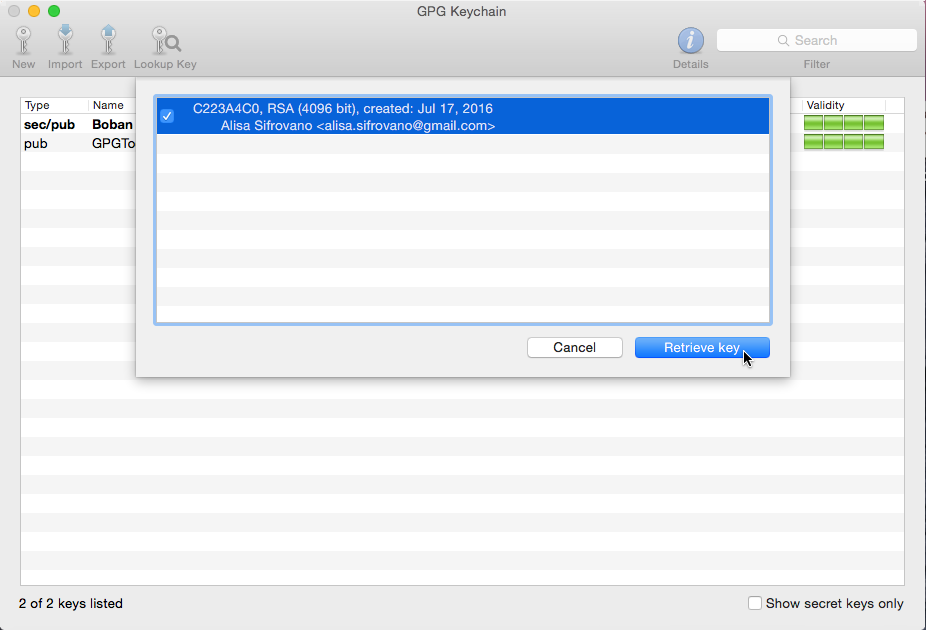
\includegraphics[width=8cm]{20_Oracle_VM_VirtualBox.png}
		\caption{ako klju\v{c} postoji, biva prona\dj{}en i mi ga preuzimamo.}
		\label{gpgtools_email_setup10}
	\end{center}
\end{figure}
\begin{figure}[!h]
	\begin{center}
		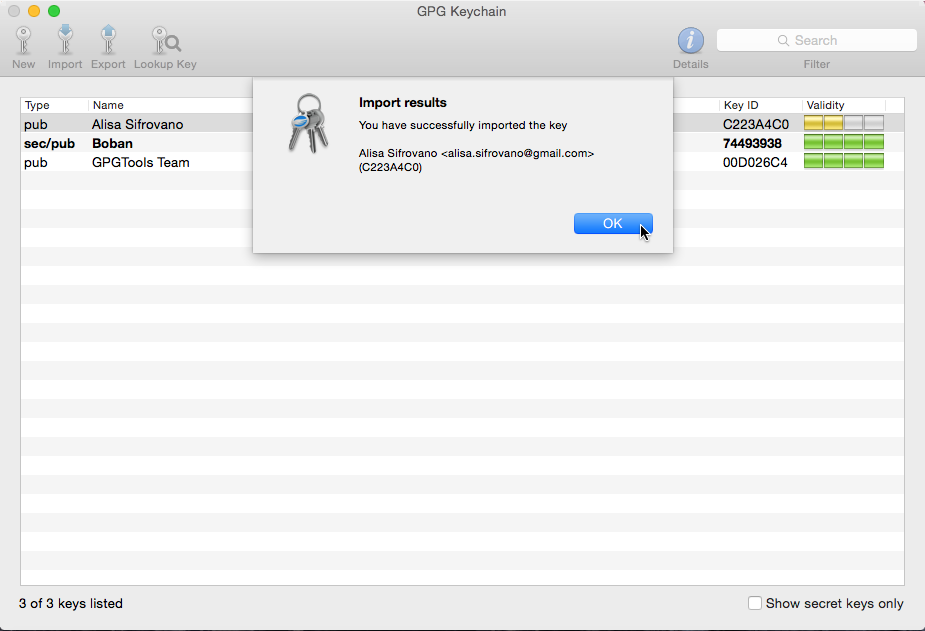
\includegraphics[width=8cm]{21_Oracle_VM_VirtualBox.png}
		\caption{Poruka o uspe\v{s}nom pribavljanju javnog novog javnog klju\v{c}a.}
		\label{gpgtools_email_setup11}
	\end{center}
\end{figure}
\newpage
\begin{figure}[!h]
	\begin{center}
		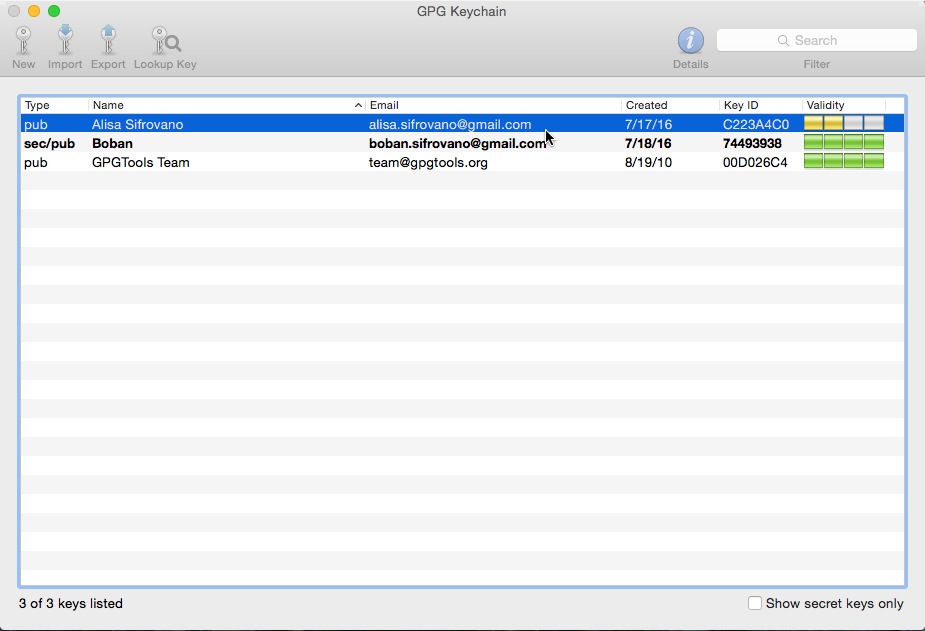
\includegraphics[width=8cm]{22_Oracle_VM_VirtualBox.png}
		\caption{Vide\'{c}e te novi klju\v{c} u \textbf{Gpgtools} programu.}
		\label{gpgtools_email_setup12}
	\end{center}
\end{figure}
\begin{figure}[!h]
	\begin{center}
		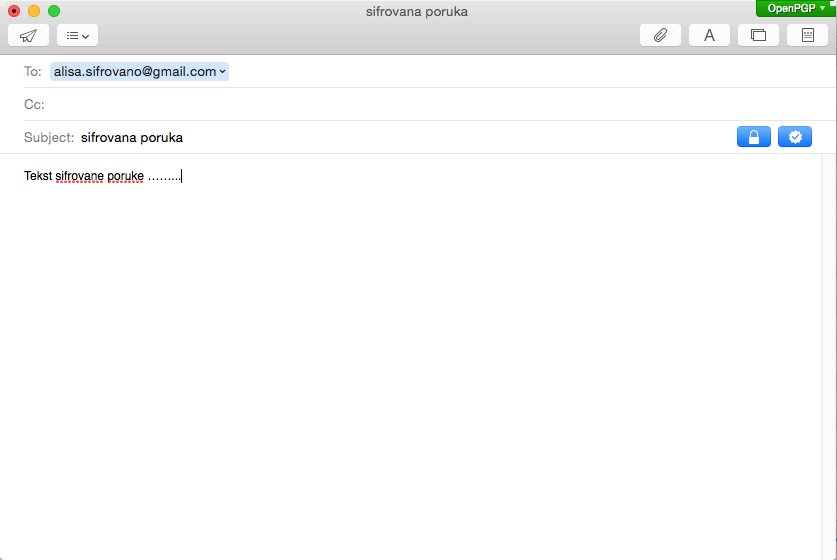
\includegraphics[width=8cm]{23_Oracle_VM_VirtualBox.png}
		\caption{I sada kada se vratimo na sastavljanje na\v{s}eg \v{s}ifrovanog mejla, posle unosa adrese primaoca poruke, vide\'{c}e te da se katanac promenio u plavu boju i da sada poruka mo\v{z} da se \v{s}ifruje.}
		\label{gpgtools_email_setup13}
	\end{center}
\end{figure}
\newpage

\begin{figure}[!h]
	\begin{center}
		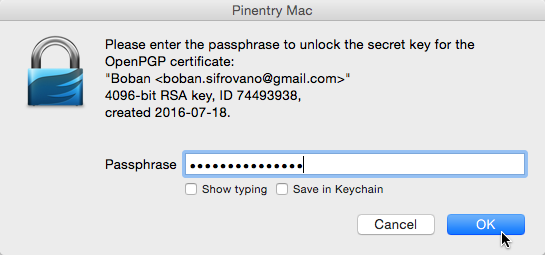
\includegraphics[width=8cm]{24_Oracle_VM_VirtualBox.png}
		\caption{Kada zavr\v{s}ite pisanje poruke i kliknete na dugme za slanje \newline(ikonica papirnog avion\v{c}i\'{c}a), tra\v{z}i\'{c}e vam \v{s}ifru za \textbf{GPG}, kako bi otklju\v{c}ao va\v{s} tajni klju\v{c} i njime digitalno potpisao poruku koju \v{s}aljete.}
		\label{gpgtools_email_setup14}
	\end{center}
\end{figure}
\section{\v{S}ta vidi mejl provajder}
\begin{figure}[!h]
	\begin{center}
		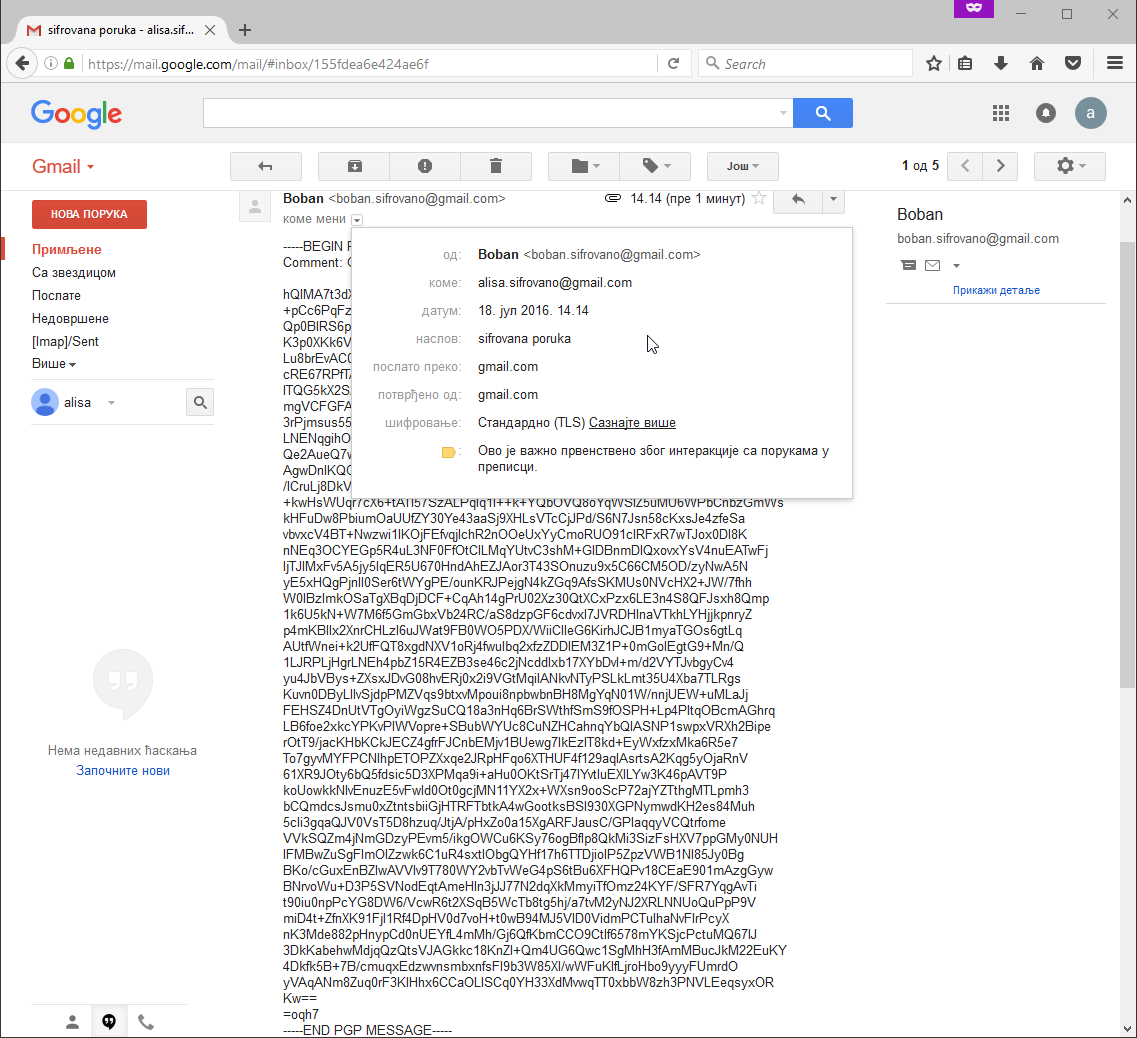
\includegraphics[width=9cm]{25_Oracle_VM_VirtualBox.png}
		\caption{Va\v{s} mejl provajder, kao i mejl provajder osobe kojoj ste poslali \v{s}ifrovanu poruku mogu videti samo naslov poruke i ko kome \v{s}alje \v{s}ifrovanu poruku, ali ne i sadr\v{z}aj iste.}
		\label{gpgtools_email_setup15}
	\end{center}
\end{figure}
\newpage
\section{De\v{s}ifrovanje primljene \v{s}ifrovane poruke}
\begin{figure}[!h]
	\begin{center}
		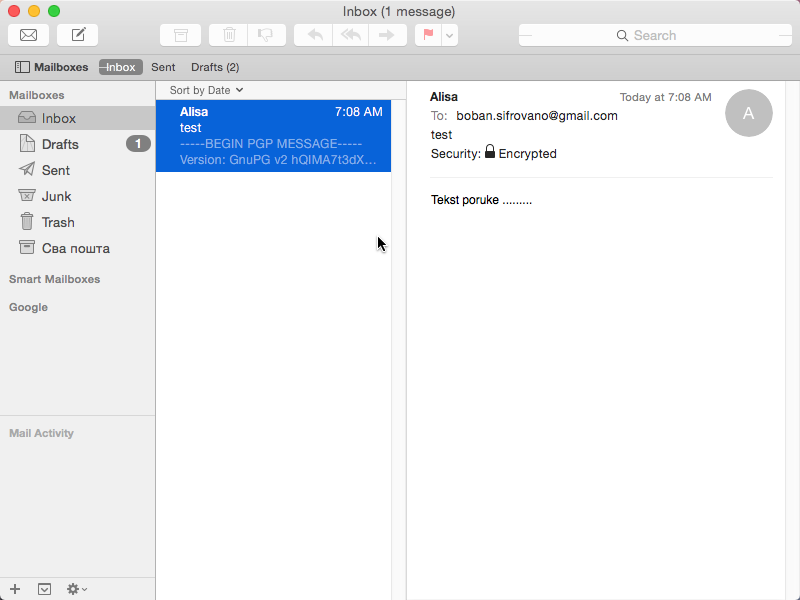
\includegraphics[width=8cm]{26_Oracle_VM_VirtualBox.png}
		\caption{Kada primite novu poruku u mejl klijentu, ako je ona \v{s}ifrovana klijent \'{c}e to prepoznati i ponuditi da de\v{s}ifruje automatksi ako unesete \v{s}ifru za va\v{s} tajni \textbf{GPG} klju\v{c}.}
		\label{gpgtools_email_setup16}
	\end{center}
\end{figure}
\end{document}
